\documentclass[tikz,border=10pt]{standalone}
\usetikzlibrary{calc}
\begin{document}
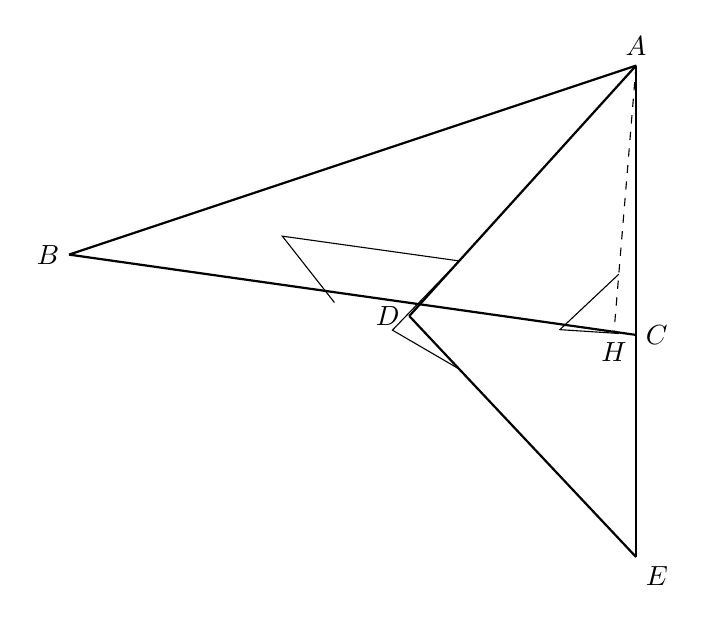
\begin{tikzpicture}[scale=1.2]
\coordinate (B) at (0,2.2);
\coordinate (D) at (3.6,1.55);
\coordinate (C) at (6.0,1.35);
\coordinate (A) at (6.0,4.2);
\coordinate (E) at (6.0,-1.0);
\coordinate (H) at ($(C)!(A)!(D)$);

\draw[thick] (B) -- (C);
\draw[thick] (B) -- (A);
\draw[thick] (A) -- (D);
\draw[thick] (D) -- (E);
\draw[thick] (A) -- (E);
\draw[dashed] (A) -- (H);

% right angle marks at H
\draw ($(H)!0.22!(C)$) -- ($($(H)!0.22!(C)$)!0.22!90:(A)$) -- ($(H)!0.22!(A)$);

% right angle marks at D (two squares)
\draw ($(D)!0.22!(B)$) -- ($($(D)!0.22!(B)$)!0.22!90:(A)$) -- ($(D)!0.22!(A)$);
\draw ($(D)!0.22!(E)$) -- ($($(D)!0.22!(E)$)!0.22!90:(A)$) -- ($(D)!0.22!(A)$);

\node[above] at (A) {$A$};
\node[left] at (B) {$B$};
\node[left] at (D) {$D$};
\node[right] at (C) {$C$};
\node[below right] at (E) {$E$};
\node[below] at (H) {$H$};
\end{tikzpicture}
\end{document}
